\subsection{Examples}

We now present some examples where we use Theorem \ref{thm_positive_rank} to force positive rank. Throughout we will consider an elliptic curve $E$ defined over $\bQ$, and a finite Galois extension $F / \bQ$ with Galois group $G = \Gal(F / \bQ)$. As described in Remark \ref{rephrase-thm}, the strategy is to find $\rho \in \R(G)$ and a $\rho$-relation $\Theta \in \B(G)$ such that $C(\Theta)$ is either not a norm from a quadratic subfield of $\bQ(\rho)$, or not a rational square, as appropriate. 

\begin{rem}[Taking quotients]
    Let $E$, $F$, $G$ be as above. Consider $H \leq G$, and $N \triangleleft G$ such that $N \leq H$. Then $C(H) = C_{E / F^H}$ is equal to $C(NH/N) = C_{E / L^{NH/N}}$ (viewing $C$ as a function on $\B(G / N)$) as the fields $F^H$ and $L^{NH/ N}$ are isomorphic. 
    
    Consider $\rho \in \R(G)$ with $N \leq \ker \rho$, so that $\bQ(\rho) = \bQ(\rho^N)$. Then, if $\Theta = \sum_i n_i H_i \in \B(G)$ with $N \leq H_i$ for all $i$, it follows that $N \cdot \Theta / N = \Theta / N$ being a norm relation for $C \colon \B(G / N) \to \bQ^{\times}$ implies that $\Theta$ is a norm relation for $C \colon \B(G) \to \bQ^{\times}$. 
\end{rem}

We will need to be able to count primes and compute residue degrees in intermediate extensions of $F / \bQ$, which is described by the following result. 

\begin{prop}[Counting primes and ramification degrees]
Consider a prime $p \in \bQ$ and decomposition and inertia groups $D_p$, $I_p \leq G$. Let $H \leq G$. 
\begin{enumerate}
    \setlength\itemsep{0em}
    \item The number of primes above $p$ in $F^H$ is given by the number of orbits of $D_p$ on $H \backslash G$, where $D_p$ acts by $d(Hg) = H g d^{-1}$ for $d \in D_p$. Equivalently it is $|H \backslash G / D_p|$.
    \item The inertia degree of a prime $\fP$ above $p$ in $F^H$ is the size of the $I_p$ sub-orbits on $H \backslash G$. 
\end{enumerate}
\end{prop}

\begin{proof}
    {\color{red} reference somewhere....}
\end{proof}


\begin{example}[Brauer relation forces growth]
    Let $G = C_2 \times C_6$, with subgroup diagram
    \begin{figure}[H]
        \centering
    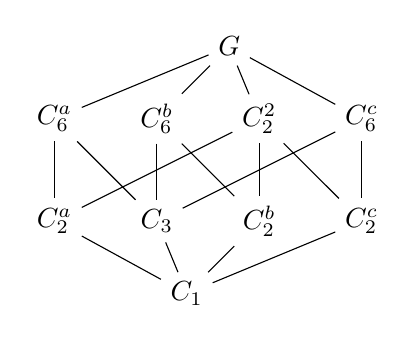
\begin{tikzpicture}[node distance=1.3cm]
        \node(G)[midway]{$G$};
        \node(C6b)[below left of =G]{$C_6^{b}$}; \node(C6a)[left of=C6b]{$C_6^{a}$};  
        \node(C22)[right of=C6b]{$C_2^{2}$};    \node(C6c)[right of=C22]{$C_6^{c}$};
        \node(C2a)[below of=C6a]{$C_2^{a}$};    \node(C3)[below of=C6b]{$C_3$};
        \node(C2b)[below of=C22]{$C_2^{b}$};    \node(C2c)[below of=C6c]{$C_2^{c}$};
        \node(C1)[below left of=C2b]{$C_1$};
        \draw(G)--(C6a);    \draw(G)--(C6b);    \draw(G)--(C6c);    \draw(G)--(C22);
        \draw(C6a)--(C2a);  \draw(C6a)--(C3);
        \draw(C6b)--(C2b);  \draw(C6b)--(C3);
        \draw(C6c)--(C2c);  \draw(C6c)--(C3);
        \draw(C22)--(C2a);  \draw(C22)--(C2b);  \draw(C22)--(C2c);
        \draw(C2a)--(C1);   \draw(C2b)--(C1);   \draw(C2c)--(C1);   \draw(C3)--(C1); 
    \end{tikzpicture}
    \end{figure}
    There is a Brauer relation coming from the $C_2 \times C_2$-quotient, given by $$\Psi = C_3 - C_6^a - C_6^b - C_6^c + 2G.$$ Consider an order $6$ character $\rho_a$ of $G$ with $C_2^{a}$ in its kernel. This has $\bQ(\rho_a) = \bQ(\zeta_6) = \bQ(\zeta_3) = \bQ(\sqrt{-3})$. Then $$\Theta = C_2^{a} - C_6^{a} - C_2^{2} + G$$ is a $\rho_a$-relation, with $\bC[ G / \Theta] = \repnorm{\rho_a}$. 

    Let $E / \bQ$ be a semistable elliptic curve and $F / \bQ$ an abelian extension with $G = \Gal(F / \bQ)$. We claim that $C(\Theta) \in \fieldnorm{\rho_a}$, for all such $E$. Since each subgroup in $\Theta$ contains $C_2^{a}$, we have that $C(\Theta)$ equals $C(\Theta / C_2^{a})$ where $\Theta / C_2^{a} \in \B(G / C_2^{a}) = \B(C_6)$.  Now $\Theta / C_2^{a}$ is a $\chi_6$-relation, where $\chi_6 = \rho_a^{C_2^a}$ is a faithful order $6$ character of $C_6$, with $\bQ(\chi_6) = \bQ(\rho_a)$. But for cyclic groups we always get norm relations; by Theorem \ref{thm_consistent_cyclic}, $C(\Theta / C_2^{a}) \in \fieldnorm{\rho_a}$.

    On the other hand, $C(\Theta + \Psi) = C(\Theta)C(\Psi)$ is not always a norm. Indeed suppose $E / \bQ$ has split multiplicative reduction at a prime $p$ with $D_p = G$, $I_p = C_6^b$ (assuming tamely ramified, one can take a prime $p$ such that $6 \mid p^2 - 1$, e.g. $p = 5$). Let $\ord_p(\Delta_E) = n$. Then there is only one prime above $p$ in each subfield, and the Tamagawa number at a prime $\fP$ above $p$ in $F^H$ is given by $c_{\fP}(E / F^H) = e_{\fP / p} n$. Suppose $E$ has good reduction at all other primes ({\color{red} or be more lenient}).
     Then 
        $$C(\Theta) = \frac{(6n)(n)}{(2n) (3n)} = 1, \qquad
            C(\Psi) = \frac{(2n)(n)^2}{(2n)(n)(2n)} = \frac{1}{2} \cdot \square.$$
    Thus $C(\Theta + \Psi) = \frac{1}{2} \mod \bQ^{\times 2}$, but $2$ is not a norm in $\bQ(\sqrt{-3})$. Hence one must have $\rk E / F > 0$. 
\end{example}

\begin{example}[Semi-direct product]
    Let $q_1$, $q_2$ be odd primes with $q_1, q_2 \equiv 1 \pmod 4$. Consider $G = C_{q_1 q_2} \ltimes C_4$ with $C_{q_1 q_2} \triangleleft G$ and $C_4$ acting faithfully on $C_{q_1 q_2}$, $C_{q_1}$, and $C_{q_2}$. This is a semidirect product by an abelian group, and its irreducible representations are described in \cite[Chapter 8, \S8.2]{Serre}. There is an irreducible representation $\rho \in \R(G)$, obtained by inducing a linear order $q_1 q_2$ faithful representation from $C_{q_1 q_2}$. Thus $\rho$ is of degree $4$ and $\bQ(\rho) = \bQ(\zeta_{q_1 q_2})^{C_4}$. Then $\rho$ has $\frac{(q_1 - 1)(q_2 - 1)}{4}$ Galois conjugates in $\R(G)$, and so $\repnorm{\rho}$ is of dimension $4 \cdot \frac{(q_1 - 1)(q_2 - 1)}{4}$. There is a $\rho$-relation $$\Theta = C_4 - (C_{q_1} \ltimes C_4) - (C_{q_2} \ltimes C_4) + G, \qquad \bC[G / \Theta] \simeq \repnorm{\rho}.$$ 

    Suppose that $E / \bQ$ is semistable. Recall that $C(\Theta) = \prod_p T_{\fP \mid p}(\Theta)$, where $T_{\fP \mid p}$ depends on $D_p$, $I_p$, the decomposition group and inertia group at $p$ respectively. Suppose that $E / \bQ_p$ has split multiplicative reduction. Ranging over all possible $D_p$ and $I_p$, a case by case analysis yields that $T_{\fP \mid p}(\Theta)$ is non-square only when $D_p = C_{q_1} \ltimes C_4$ or $C_{q_2} \ltimes C_4$ (and $I_p$ is non-trivial). 

    For example, let $D_p = C_{q_1} \ltimes C_4$, $I_p = C_{q_1}$.
        \begin{itemize}[--]
            \setlength\itemsep{0em}
            \item The action of $D_p$ on $C_4 \backslash G$ yields $1$ orbit of size $C_{q_1}$ (the orbit of the identity) and $\frac{q_2 - 1}{4}$ orbits of size $4q_1$ (coming from $C_4$ acting faithfully on $C_{q_2}$). The size of the inertia sub-orbits is $q_1$. Hence $T_{\fP \mid p}(C_4) = (q_1 n)^{1 + \frac{q_2 - 1}{4}}$.
            \item The action of $D_p$ on $C_{q_1} \ltimes C_4 \backslash G$ yields the same number of orbits as above, but now the action of $C_{q_1} \leq D_p$ is trivial and the size of the inertia sub-orbits are all $1$, so that $T_{\fP \mid p}(C_{q_1} \times C_4) = n^{1 + \frac{q_2 - 1}{4}}$.
            \item The action of $D_p$ on $C_{q_2} \ltimes C_4 \backslash G$ yields one orbit of size $q_1$, with the inertia sub-orbit also of size $q_1$, hence $T_{\fP \mid p}(C_{q_2} \times C_4) = q_1 n$.
        \end{itemize}
    Hence
    \[ T_{\fP \mid p}(\Theta) = \frac{(q_1 n )^{1 + \frac{q_2 - 1}{4}} (n)}{(n)^{1 + \frac{q_2 - 1}{4}} (q_1 n)} = q_1^{\frac{q_2 - 1}{4}} .\] 
    By symmetry, taking $D_p = C_{q_2} \ltimes C_4$, $I_p = C_{q_2}$, one has $T_{\fP \mid p}(\Theta) = q_2^{\frac{q_1 - 1}{4}}$.

    So let $E / \bQ$ have split multiplicative reduction at $p$ with $D_p = C_{q_1} \ltimes C_4$, $I_p = C_{q_1}$, and good reduction at all other primes. Suppose that $q_2 \not\equiv 1 \pmod 8$ and that $\legendre{q_1}{q_2} = -1$. Then $\bQ(\sqrt{q_1 q_2}) \subset \bQ(\rho)$ but $T_{\fP \mid p}(\Theta) \not\in N_{\bQ(\sqrt{q_1 q_2}) / \bQ}(\bQ(\sqrt{q_1 q_2})^{\times})$. One has $T_{\fP \mid p}(\Theta) \equiv q_1 \mod \bQ^{\times 2}$, but $q_1$ is not the norm of an element of $\bQ(\sqrt{q_1 q_2})$. 
    If it were, then there would exist $x, y, z \in \bZ$ such that $z^2 q_1 = x^2 - q_1 q_2 y^2$. Looking mod $q_2$ this implies that $q_1 = \square \pmod {q_2}$, a contradiction. Thus $\rk E / F > 0$ by Theorem \ref{thm_positive_rank}. For example, one can take $q_1 = 17$, $q_2 = 5$. 

    This rank growth is predicted by root number computations also, however. Assume that $F / \bQ$ is totally real. Then $w(E / F^H) = (-1)^{[F^H : \bQ] + | H \backslash G / D_p|}$. Thus {\color{red} I need to introduce these somewhat somewhere}
    \begin{itemize}[--]
        \setlength\itemsep{0em}
        \item $w(E / \bQ) = (-1)^2 = 1$,
        \item $w(E / F^{C_4}) = (-1)^{q_1 q_2} (-1)^{1 + \frac{q_2 - 1}{4}} = (-1)^{\frac{q_2 - 1}{4}}$,
        \item $w(E / F^{C_{q_1} \ltimes C_4}) = (-1)^{q_2}(-1)^{1 + \frac{q_2 - 1}{4}} = (-1)^{\frac{q_2 - 1}{4}},$
        \item $w(E / F^{C_{q_2} \ltimes C_4}) = (-1)^{q_1}(-1) = 1$. 
    \end{itemize}
    Therefore if $q^2 \not\equiv 1 \pmod 8$, we must have $\rk E / F^{C_4}, \rk E / F^{C_{q_1} \ltimes C_4} > 0$, so $\rk E / F > 0$. Note that we needed to additionally assume that $\legendre{q_1}{q_2} = -1$, but the root number computation doesn't need this assumption. For example, if $q_1 = 29$, $q_2 = 5$, then $5 = (\frac{15}{4})^2 - 29*5(\frac{1}{4})^2$ is a norm from $\bQ(\sqrt{5 \cdot 29})$, so we can't use Theorem \ref{thm_positive_rank}. 
\end{example}

\begin{example}[Additive reduction example]

\end{example}